\subsection{Reading Edgelist from text file}

We attempt a number of approaches to read Edgelist from text file into in-memory Edgelist(s), given in Sections \ref{sec:el-fstream-plain}-\ref{sec:el-mmap-custom}. Among these, we find using \texttt{mmap()} with custom number parsers (\textit{mmap-custom}) to be the best approach. The pseudocode for \textit{mmap-custom} is given Algorithm \ref{alg:el}.


\subsubsection{\texttt{ifstream} with \texttt{getline()} and \texttt{>>} operator (\textit{fstream-plain})}
\label{sec:el-fstream-plain}

In this approach, we utilize C++'s \texttt{ifstream} to open the file, and read the edges line by line with \texttt{getline()}. If the graph is unweighted, we read the source and target vertex ids as 64-bit unsigned integers, using \texttt{>>} operator, into pre-allocated source and target arrays based on information in the file header. If the graph is weighted, we also read the weights as 32-bit floating-point numbers into another pre-allocated array. This process is sequential, given that streams are inherently sequential.


\subsubsection{\texttt{ifstream} with \texttt{getline()} and \texttt{strto*()} (\textit{fstream-strto*})}
\label{sec:el-fstream-stro*}

In this approach, we again use \texttt{ifstream} but employ string-to-number conversion methods \texttt{strtoull()} and \texttt{strtod()} for parallel number parsing. We sequentially read a block of $L$ lines from the file, using \texttt{getline()}, and then parse each line in parallel using multiple threads. We observe that using OpenMP's dynamic scheduling, with a chunk size of $1024$, and reading a block of $L=128K$ lines to be processed in parallel offers the best performance. Parsed edges (source, target vertex ids, and edge weights) are stored separately in per-thread edge lists to avoid contention issues within a shared data structure. With 64 threads, this approach demonstrates a speedup of $8.7\times$ compared to \textit{fstream-plain}, as shown in Figure \ref{fig:optimize-el}.

\begin{figure}[hbtp]
  \centering
  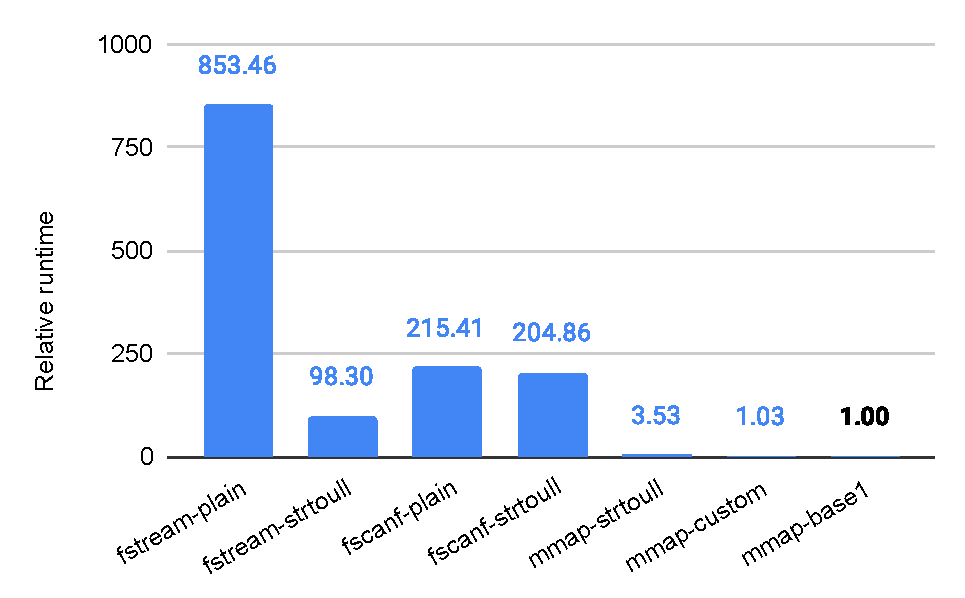
\includegraphics[width=0.99\linewidth]{out/optimize-el.pdf} \\[-2ex]
  \caption{Gini coefficient of PageRank values on 24 different graphs, comparing between PageRank values obtained with three different dead-end handling strategies: \textit{teleport from dead-ends} (\textbf{default}), \textit{self-loop dead-ends} (\textbf{loop}), and \textit{self-loop all vertices} (\textbf{loopall}).}
  \label{fig:optimize-el}
\end{figure}



\subsubsection{\texttt{fopen()} with \texttt{fgets()} and \texttt{sscanf()} (\textit{fopen-plain})}
\label{sec:el-fopen-plain}

This approach is similar to the one mentioned above (\textit{fscanf-strto*}), but we use \texttt{fgets()} on a file handle to read lines instead of \texttt{getline()}, and employ \texttt{sscanf()} to parse the edges. With 64 threads, it provided a speedup of $4.0\times$ compared to \textit{fstream-plain}.


\subsubsection{\texttt{fopen()} with \texttt{fgets()} and \texttt{strto*()} (\textit{fopen-strto*})}
\label{sec:el-fopen-strto*}

Similar to the previous approach (\textit{fopen-plain}), this one uses \texttt{fgets()} to read lines from the text file, but replaces \texttt{sscanf()} with \texttt{strtoull()} and \texttt{strtod()}. This proves faster due to the absence of a format string. At 64 threads, its speedup is $1.1\times$ over \textit{fopen-plain}.


\subsubsection{\texttt{mmap()} with \texttt{strto*()} (\textit{mmap-strto*})}
\label{sec:el-mmap-strto*}

In this approach, we map the file to memory with \texttt{mmap()}, and process the edges in parallel by partitioning the file into blocks of $C$ characters. Each block is dynamically assigned (using OpenMP's dynamic schedule) to a free thread. If the assigned block contains partial lines at either end, the thread repositions it, by shifting to the right to eliminate partial lines. This involves skipping the partial line at the beginning and including the partial line from the end. We observe that issuing \texttt{madvice(MADV\_WILLNEED)}, and using a block size of $\beta=256K$ characters offers the best performance. To parse the source/target vertex ids and edge weights, we use \texttt{strtoull()} and \texttt{strtod()}. Each thread stores the parsed edges in per-thread Edgelists. With 64 threads, it provides a speedup of $58.5\times$ over \textit{fopen-strto*}, as show in Figure \ref{fig:optimize-el}.


\subsubsection{\texttt{mmap()} with custom number parsers (\textit{mmap-custom})}
\label{sec:el-mmap-custom}

This is similar to the approach mentioned above (\textit{mmap-strto*}), but we use our own functions for parsing whole numbers and floating-point numbers. In addition, as vertex ids start with $1$, we decrement $1$ from the vertex ids after parsing it and before appending them to per-thread Edgelists. Surprisingly, this leads to $40-50\%$ drop in performance. Converting the $weighted$ flag (see Algorithm \ref{alg:el}) to a template parameter solves this issue. This indicates that the issue was related to the loop code not being able to fit in the code cache of the processor and using a template allowed it to fit in the cache. Accordingly, we also recommend using $symmetric$ flag as a template parameter instead. With 64 threads, it provides a speedup of $3.5\times$ over \textit{mmap-strto*}. We also attempted to use custom SIMD instructions to parse numbers, along with \texttt{vzeroupper} instruction to clear SSE/AVX registers, but it did not provide additional performance improvement.

\begin{algorithm}[hbtp]
\caption{Reading Edge-list from file.}
\label{alg:el}
\begin{algorithmic}[1]
\Require{$pdegrees$: Per partition vertex degrees (output)}
\Require{$edges$: Per thread sources, targets, and weights of edges (output)}
\Require{$data$: Memory mapped file data}
\Ensure{$counts$: Number of edges read per thread (output)}
\Ensure{$symmetric$: Is graph symmetric?}
\Ensure{$weighted$: Is graph weighted?}
\Ensure{$\beta$: Size of each block that is processed per thread}
\Ensure{$\rho$: Number of partitions for counting vertex degrees}
\Ensure{$t$: Current thread}

\Statex

\Function{getBlock}{$data, i$} \label{alg:frontier--main-begin}
  \State $[d, D] \gets data$
  \State $b \gets d+i$ \textbf{;} $B \gets min(b+\beta, D)$
  \If{$b \neq d$ \textbf{and not} $isNewline(b-1)$}
    \State $b \gets findNextLine(b, D)$
  \EndIf
  \If{$B \neq d$ \textbf{and not} $isNewline(B-1)$}
    \State $B \gets findNextLine(B, D)$
  \EndIf
  \Return{$[b, B]$}
\EndFunction

\Statex
  
\Function{readEdgelist}{$pdegrees, edges, data$}
  \State $counts \gets \{0\}$
  \State $[sources, targets, weights] \gets edges$
  \State $\rhd$ Load edges from text file in blocks of size $\beta$
  \ForAll{$i \in [0, \beta, 2\beta, ... |data|]$ \textbf{in parallel}}
    \State $j \gets counts[t]$
    \State $[b, B] \gets getBlock(data, i)$
    \While{$true$}
      \State $\rhd$ Read an edge from the block
      \State $u \gets v \gets 0$ \textbf{;} $w \gets 1$
      \State $b \gets findNextDigit(b, B)$
      \If{$b = B$} \textbf{break}
      \EndIf
      \State $b \gets parseWholeNumber(u, b, B)$
      \State $b \gets findNextDigit(b, B)$
      \State $b \gets parseWholeNumber(v, b, B)$
      \If{$weighted$}
        \State $b \gets findNextDigit(b, B)$
        \State $b \gets parseFloat(w, b, B)$
      \EndIf
      \State $\rhd$ Make it zero-based
      \State $u \gets u - 1$ \textbf{;} $v \gets v - 1$
      \State $\rhd$ Add the parsed edge to edgelist
      \State $sources[t][j] \gets u$
      \State $targets[t][j] \gets v$
      \If{$weighted$} $weights[t][j] \gets w$
      \EndIf
      \State $atomicAdd(pdegrees[t \bmod \rho][u], 1)$
      \State $j \gets j + 1$
      \State $\rhd$ If graph is symmetric, add the reverse edge
      \If{$symmetric$}
        \State $sources[t][j] \gets v$
        \State $targets[t][j] \gets u$
        \If{$weighted$} $weights[t][j] \gets w$
        \EndIf
        \State $atomicAdd(pdegrees[t \bmod \rho][v], 1)$
        \State $j \gets j + 1$
      \EndIf
    \EndWhile
    \State $counts[t] \gets j$
  \EndFor
  \Return{$counts$}
\EndFunction
\end{algorithmic}
\end{algorithm}

\begin{algorithm}[hbtp]
\caption{Convert Edge-list to CSR.}
\label{alg:csr}
\begin{algorithmic}[1]
\Require{$csr$: Global CSR (output)}
\Require{$pcsr$: Per partition CSR (scratch)}
\Require{$pdegrees$: Per partition vertex degrees (scratch)}
\Require{$edges$: Per thread sources, targets, and weights of edges}
\Require{$counts$: Number of edges read per thread}
\Ensure{$symmetric$: Is graph symmetric?}
\Ensure{$weighted$: Is graph weighted?}
\Ensure{$\rho$: Number of partitions for counting vertex degrees}
\Ensure{$t$: Current thread}

\Statex

\Function{convertToCsr}{$csr, pcsr, pdegrees, edges, counts$}
  \State $[offsets, edgeKeys, edgeValues] \gets csr$ \label{alg:csr--initialize-begin}
  \State $[poffsets, pedgeKeys, pedgeValues] \gets pcsr$
  \State $[sources, targets, weights] \gets edges$ \label{alg:csr--initialize-end}
  \State $\rhd$ Compute offsets
  \ForAll{$p \in [0, \rho)$} \label{alg:csr--poffsets-begin}
    \State $exclusiveScan(poffsets[p], pdegrees[p], |V|+1)$
  \EndFor \label{alg:csr--poffsets-end}
  \State $\rhd$ Populate per-partition CSR
  \ForAll{\textbf{threads in parallel}} \label{alg:csr--pcsr-begin}
    \ForAll{$i \in [0, counts[t])$}
      \State $u \gets sources[t][i]$
      \State $v \gets targets[t][i]$
      \State $j \gets atomicAdd(poffsets[t \bmod \rho][u], 1)$
      \State $pedgeKeys[t \bmod \rho][j] \gets v$
      \If{$weighted$}
        \State $pedgeValues[t \bmod \rho][j] \gets weights[t][i]$
      \EndIf
    \EndFor
  \EndFor \label{alg:csr--pcsr-end}
  \State $\rhd$ Fix per-partition offsets
  \ForAll{\textbf{threads in parallel}} \label{alg:csr--poffsets-fix-begin}
    \If{$t < \rho$}
      \State $memcpy(poffsets[t]+1, poffsets[t], |V|)$
      \State $poffsets[t][0] \gets 0$
    \EndIf
  \EndFor \label{alg:csr--poffsets-fix-end}
  \State $\rhd$ Combine per-partition degrees
  \ForAll{$u \in [0, |V|)$ \textbf{in parallel}} \label{alg:csr--poffsets-combine-begin}
    \ForAll{$p \in [1, \rho)$}
      \State $pdegrees[0][u] +\gets pdegrees[p][u]$
    \EndFor
  \EndFor \label{alg:csr--poffsets-combine-end}
  \State $\rhd$ Compute global offsets
  \State $exclusiveScan(offsets, pdegrees[0], |V|+1)$ \label{alg:csr--offsets-compute}
  \State $\rhd$ Combine per-partition CSR into one CSR
  \ForAll{$u \in [0, |V|)$ \textbf{in parallel}} \label{alg:csr--pcsr-combine-begin}
    \State $j \gets offsets[u]$
    \ForAll{$p \in [0, \rho)$}
      \State $i \gets poffsets[t][u]$
      \State $I \gets poffsets[t][u+1]$
      \ForAll{$i \in [i, I)$}
        \State $edgeKeys[j] \gets pedgeKeys[t][i]$
        \If{$weighted$}
          \State $edgeValues[j] \gets pedgeValues[t][i]$
        \EndIf
        \State $j \gets j + 1$
      \EndFor
    \EndFor
  \EndFor \label{alg:csr--pcsr-combine-end}
\EndFunction
\end{algorithmic}
\end{algorithm}


The psuedocode of the \textit{mmap-custom} approach is given in Algorithm \ref{alg:el}. It loads per-thread Edgelists from a file with the best performance, and is enacpsulated in the \texttt{readEdgelist()} function\ignore{(lines \ref{alg:el--read-edgelist-begin}-\ref{alg:el--read-edgelist-end})}. First, the counts of edges read per thread ($counts$) are initialized, and the components of per-thread Edgelists are obtained ($edges$) in lines \ref{alg:el--initialize-begin}-\ref{alg:el--initialize-end}. This is followed by a loop (lines \ref{alg:el--blocks-begin}-\ref{alg:el--blocks-end}), where each iteration processes a block of characters (of size $\beta = 256K$) in the text file in parallel across different threads. The text file is assumed to have been memory mapped as $data$. Inside the loop, $j$ keeps track of the number of edges processed by the current thread. In line \ref{alg:el--get-block}, the \texttt{getBlock()} function is called to retrieve the begin and end of current block of text ($[b, B]$), which is processed in the main loop (lines \ref{alg:el--block-begin}-\ref{alg:el--block-begin}). The main loop parses edges (lines \ref{alg:el--parse-edge-begin}-\ref{alg:el--parse-edge-end}), adjusts vertex indices to be zero-based (line \ref{alg:el--base1}), and adds them to the Edgelist of the current thread while updating per-partition vertex degrees with atomic operations (lines \ref{alg:el--add-edge-begin}-\ref{alg:el--add-edge-end}). Reverse edges are added for symmetric graphs (lines \ref{alg:el--reverse-edge-begin}-\ref{alg:el--reverse-edge-end}). Finally, counts of processed edges per thread are recorded (line \ref{alg:el--update-counts}) and returned (line \ref{alg:el--return-counts}).

The \texttt{getBlock()} function\ignore{(lines \ref{alg:el--get-block-begin}-\ref{alg:el--get-block-begin})} retrieves a block of characters to process\ignore{from the memory-mapped file}, starting from index $i$. It ensures that the block starts and ends on newline characters for proper parsing. The block size is determined by the parameter $\beta$, which is set to $256K$.




\subsection{Converting Edgelist to CSR}

Now that we have obtained per-thread Edgelists, we must now convert the Edgelists to CSR. We attempt a few of approaches for this in steps, given in Sections \ref{sec:csr-degree-global}-\ref{sec:csr-csr-partition4}. Among these, we find that obtaining CSR from vertex degrees, where the vertex degrees are computed in four separate partitions using $\bmod$ operator with the current thread id, performs the best. The pseudocode for \textit{csr-partition4} is given in Algorithm \ref{alg:csr}.


\subsubsection{Obtain global vertex degrees along with reading Edgelist (\textit{degree-global})}
\label{sec:csr-degree-global}

To convert the Edgelists to CSR, we first need to know the degree of each vertex. In this approach, we use a simple solution for this, i.e.,  we update the degree of each vertex in a single shared array using atomic operations, while reading Edgelists on each thread. The relative runtime of this approach with respect to simply reading per-thread Edgelists is $1.9\times$, as shown in Figure \ref{fig:optimize-csr}. We however observe that this results in high contention and impacts performance.

\begin{figure}[hbtp]
  \centering
  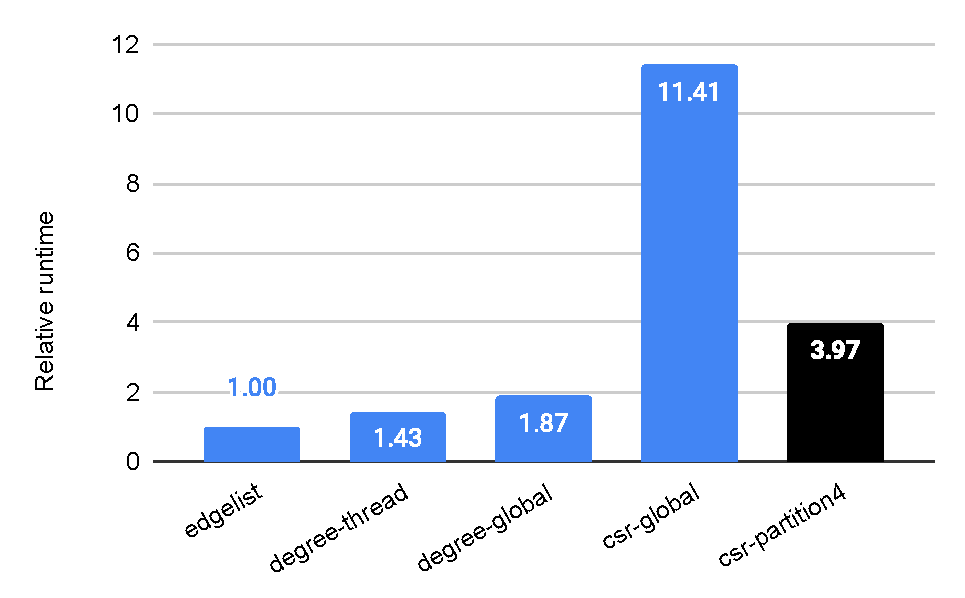
\includegraphics[width=0.99\linewidth]{out/optimize-csr.pdf} \\[-2ex]
  \caption{Gini coefficient of PageRank values on 24 different graphs, comparing between PageRank values obtained with three different dead-end handling strategies: \textit{teleport from dead-ends} (\textbf{default}), \textit{self-loop dead-ends} (\textbf{loop}), and \textit{self-loop all vertices} (\textbf{loopall}).}
  \label{fig:optimize-csr}
\end{figure}



\subsubsection{Obtain per-thread vertex degrees along with reading Edgelist (\textit{degree-thread})}
\label{sec:csr-degree-thread}

In this approach, we compute per-thread vertex degrees instead of global degrees. While this improves performance by $24\%$ compared to obtaining global vertex degrees, it requires significant additional space, and needs to be combined later to obtain global degrees. We observe that computing degrees in partitions of $4$ (using $\bmod 4$) and then combining them into a global degrees array gives us the best performance.


\subsubsection{Obtain CSR from global vertex degrees (\textit{csr-global})}
\label{sec:csr-csr-global}

Now that we have the degrees, we need to combine the per-thread Edgelists into a CSR data structure. In this approach, we first obtain global vertex degrees along with reading per-thread Edgelists (as with \textit{degree-global}), and then convert the per-thread Edgelists to a global CSR in parallel using atomic operations. As shown in Figure \ref{fig:optimize-csr}, this approach has poor performance (it is $11.4\times$ slower than simply reading Edgelists).


\subsubsection{Obtain CSR from 4-partitioned vertex degrees (\textit{csr-partition4})}
\label{sec:csr-csr-partition4}

Finally, we explore computing CSR in $k$ separate partitions and later combining them into a single global CSR. The vertex degrees are also obtained in $k$ partitions while reading Edgelist, which is then used for generating partitioned CSR. We adjust the value of $k$ from $1$ to $16$. Our observations indicate that using $4$ partitions to generate CSR and then combining them has the best performance - it offers $2.9\times$ speedup over \textit{csr-global}.

The psuedocode of the \textit{csr-partition4} approach is given in Algorithm \ref{alg:csr}. It transforms an Edgelist representation of a graph into CSR format. First, the components of global CSR ($csr$), per-partition CSRs ($pcsr$), and per-thread Edgelists ($edges$) are obtained in lines \ref{alg:csr--initialize-begin}-\ref{alg:csr--initialize-end}. The algorithm then computes offsets for each partition in parallel (lines \ref{alg:csr--poffsets-begin}-\ref{alg:csr--poffsets-begin}) using exclusive scan operations, and updates the per-partition CSRs concurrently (lines \ref{alg:csr--pcsr-begin}-\ref{alg:csr--pcsr-end}). Atomic operations ensure thread safety when updating the matrices. In lines \ref{alg:csr--poffsets-fix-begin}-\ref{alg:csr--poffsets-fix-end}, per-partition offsets are fixed as they were updated during the edge insertion process above. The algorithm then combines per-partition degrees (lines \ref{alg:csr--poffsets-combine-begin}-\ref{alg:csr--poffsets-combine-end}), computes global offsets (line \ref{alg:csr--offsets-compute}), and merges the per-partition CSRs into the global CSR (lines \ref{alg:csr--pcsr-combine-begin}-\ref{alg:csr--pcsr-combine-begin}).
